

\section{Electricity price forecasting}

A lot of research has been going on in electricity price forecasting in power markets. Different strategies and models have been developed of which the most relevant regarding this thesis will be discussed. 


\subsection{Forecasting spot electricity prices with time series models}

In \cite{weron2005forecasting} the authors state that forecasting electricity prices with accuracy levels comparable to electricity load forecasting is hard to achieve, as different seasonality patterns (e.g.~daily, weekly, annually) and exogenous variables (such as loads and network constraints) have to be taken into account. 

Three basic types of models for electricity price forecasting have been identified: 

\begin{itemize}
	\item parsimonious stochastic models
	\item structural or fundamental models
	\item non-parametric models
\end{itemize}

where focus has been laid on a combination of the first two types of models. 

Data was taken from the Californian power market from before and during the market crash in 2001. Preprocessing has been done by removing outliers (substitution by the arithmetic average of neighbouring values), mean removal (center data around zero) and logarithmic transformations of load ($z_t = \log(Z_t)$) and price ($p_t = \log(P_t)$) time series. The latter approach is used to obtain a more stable variance of the time series data. 

For building forecast models for the next 24 hours of the following day historical prices and demand as well as day ahead load predictions of the next 24 hours have been utilized. In order to model the daily variation of demand, costs and operational constraints models have been built for each hour separately which is inspired by studies of demand forecasting \cite{bunn2000forecasting}. 

To achieve seasonal autoregression models the log price $p_t$ was made dependent on the same hour in previous days and weeks as well as on an aggregate function based on the previous day prices. The system load has been used as the fundamental variable as strong correlations between loads and prices have been revealed (Figure \ref{fig:log_loads_vs_log_prices}). 

\begin{figure}[htbp]
	\centering
		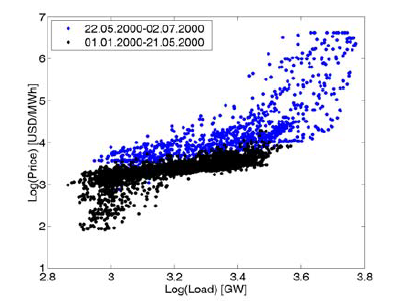
\includegraphics{figures/state_of_the_art/log_loads_vs_log_prices.PNG}
	\caption{The dependence between the
hourly log prices and hourly log system
loads in California for the period January 1
– July 2, 2000. \cite{weron2005forecasting}}
	\label{fig:log_loads_vs_log_prices}
\end{figure}

As can be observed the dependence between loads and energy prices is almost linear except for very low and very high loads, where electricity prices tend to jump to lower and higher values, respectively. 

Results show that for the proposed dataset ARX models (AR with exogenous variables) exhibit lower mean weekly errors (MWE) than AR models which in turn had significantly lower errors than standard ARIMA models. The difference is the separate modeling of individual hours for the ARX and AR models as opposed to an 48 hour aggregate modeling for ARIMA models. 

\subsection{ARIMA models to predict next-day electricity prices}

The authors in \cite{contreras2003arima} propose the application of ARIMA models for day ahead energy price forecasting based on data in the Spanish and Californian power markets. These models are based on time series analysis and results show that accurate electricity price forecasting for the aforementioned power markets is possible. Depending on the market and selected time range average weekly prediction errors 
range from 5\% to 10\%. These results are quite reasonable given that prices from the Californian market in the year 2000 have been selected which has been a very volatile and unstable time period due to the market crash in early 2001 \cite{weron2007modeling}. 

The described model generation process consists of five steps: 

\begin{itemize}
	\item[0)] A class of models is formulated assuming certain hypotheses.
	\item[1)] A model is identified for the observed data.
	\item[2)] The model parameters are estimated.
	\item[3)] If the hypotheses of the model are validated, go to Step 4, otherwise go to Step 1 to refine the model.
	\item[4)] The model is ready for forecasting.
\end{itemize}

This process is taken from the Box Jenkins methodology for forecast model generation \cite{hibon1997arma}.

Interestingly only five hour training periods are needed to model forecasts for the next consecutive hour for Spanish power prices, only two hour training periods are needed for modeling Californian energy prices. 
Through outlier detection the resulting forecasts could have been slightly improved but as stated in \cite{contreras2003arima} this would result in significantly increased computation time. 


\subsection{Energy price forecasting approaches in wholesale power markets}

According to \cite{lora2007electricity} electricity price models in general can be classified in two different sets of models, production cost models and statistical models. 

Production cost models retrieve all available information to accurately model system behavior while statistical models are trained on historical data and have little information about the underlying system. An advantage of statistical models is that the amount of information needed to build models is significantly less than that needed for production cost models. 

Statistical time series models can in turn be classified in classical time series models and models based on machine learning approaches \cite{lora2007electricity}. Classical time series models have the benefit to exhibit a simpler structure than machine learning models, however it is hard to obtain accurate forecasts for non-linear time series such as energy prices. 

Regarding machine learning approaches, artificial neural networks (ANN) have been studied extensively in relation to electricity price forecasting \cite{vahidinasab2008day, singhal2011electricity, pao2007forecasting, amjady2006day, catalao2007short, 
gareta2006forecasting, duanelectricity, szkuta1999electricity}. Neural network models are trained to model non-linear relationships between applicable input variables and historical energy prices. 

Results show that ANN models have the potential to significantly outperform statistical models such as Autoregressive (AR) or ARIMA models \cite{pao2007forecasting, catalao2007short}. This may be due to their ability to more accurately model the underlying system behavior while they excel at modeling non-linear relationships in the dataset. 

However, in order to successfully apply forecasting based on neural network models a set of requirements have to be met \cite{catalao2007short}: Availability of sufficient amounts of data, adequate selection of input/output samples, an appropriate number of hidden units and sufficient computational resources. In case these requirements can not be met or it is not possible to appropriately parametrize the model statistical models provide a good alternative for modeling energy prices. 


%Different methods have been proposed for applying load and energy price forecasting in wholesale power markets. Two basic types of models can be discerned: time series based models and computationally intensive machine learning approaches \cite{bunn2000forecasting, weron2007modeling}. 
%
%Price and load forecasting is evaluated in \cite{bunn2000forecasting} by investigating the England and Wales energy markets. 
%Forecasting daily loads is discussed based on computationally intensive methods where three types of approaches are considered:
%variable segmentation, combination of forecasts and load forecasting with neural networks.

%They point out that load forecasting is inherently different from price forecasting despite the fact that price movements are based on variations in load. Additionally research in the area of price forecasting has been still immature and needs to be investigated in depth. 

%\subsection{Forecasting Loads and Prices in Competitive Power Markets}




\subsection{Forecasting next day electricity prices by computationally intensive methods}

Some approaches were taken to provide forecast models for next day electricity prices in wholesale power markets. Basically there are two different approaches for energy price forecasting. 




\subsection{Electricity Market Price Forecasting Based on Weighted Nearest Neighbors Techniques}

\cite{lora2007electricity}


%The first step (0) consists of determining a suitable class of models that can be applied to the time series based on observed characteristics, e.g.~high frequency, nonconstant mean and variance, and multiple seasonality. The hypothesis of the model at this step assumes a forecast error term with a normal distribution having a zero mean and constant variance. 
%
%In step 1) a trial model has to be selected for which data has to be made stationary. Through application of a logarithmic transformation a more stable variance can be achieved whereas (seasonal) differencing of data may result in a more stable mean. In order to find appropriate autoregressive and moving average coefficients for the resulting ARIMA model autocorrelation (ACF) and partial autocorrelation (PACF) plots may be consulted to retrieve a first fit of the model. 
%
%Step 2) consists of estimation of parameters which is typically done by applying the maximum likelihood function with respect to the parameters. In order to optimize forecasting performance outlier detection methods may be applied to minimize the impact of single "`spikes"' in the data. 
%
%In step 3) the residuals (forecast errors) of the resulting model are evaluated based on desired characteristics. Residuals should exhibit zero mean, constant variance, should follow a normal distribution and should be uncorrelated. Suitable tests for these properties are portmanteau tests (Ljung box, Box Pierce) and examination of ACF and PACF plots to find dependencies within the data. 
%
%Step 4) is concluding the model selection process. The resulting model of step 2) is used for forecasting based on trained data. 



\section{Optimize resource scheduling in geo distributed data centers}

\section{Cost optimization in data centers}

Active research topics in this field include electricity cost reduction in data centers \cite{guler2013cutting, le2011reducing}. A comparison of different approaches considering spatial and temporal energy price changes and the contribution of the outside temperature to the resulting cooling effort and expense is outlined in \cite{guler2013cutting}. In \cite{le2011reducing} a set of homogenous data centers is simulated where the focus lies on the effects of changing workloads and migrations on the cooling infrastructure and on intelligent scheduling to reduce energy consumption and energy costs, respectively. 

The authors in \cite{lucanin2013take} propose a green cloud approach using real time electricity prices where the duration and time of price peaks are estimated and VMs are paused during these times to reduce energy costs and save energy. Customers may choose between ``green'' and normal instances, taking into account some loss of availability for a reduced price. 



In \cite{rao2010minimizing} a cloud consisting of several Internet Data Centers (IDC) is examined with regard to cost optimization which is done by intelligently assigning workload to data centers based on current energy prices. Two of these data centers in the scenario are connected to deregulated wholesale energy markets whereas the other one is connected to a regulated utility region charged by a fixed pricing scheme. Since price change differences in deregulated energy markets can be considerable energy cost reductions may be achieved by assigning workload based on changing energy prices.  %For the purpose of the simulation five front-end Web portal servers process a total workload of about $10^5$ requests per second. 

In this paper the approaches of optimal and average workload assignments are visually and formally compared to gain insights into the total electricity cost reduction. The optimal workload assignment is calculated with respect to workload and delay constraints that are considered in a minimum cost flow problem based on a linear programming model. Thus the goal is to minimize costs without compromising quality of service constraints. 
%The proposed cost reductions amount up to 30 percent for a single hour test within the given time range. 
%The results measured at two timestamps at a specific day seem promising, since total cost reductions could be achieved by 30\% and 17\% respectively. 

The differences compared to this work is that in \cite{rao2010minimizing} they do not consider longer running jobs as used in scientific calculations or large optimization problems that may take several hours to complete. Thus the impact of migrations is not examined in this scenario. In addition the possibility of energy price forecasting is not considered which may result in even greater energy cost reductions. 

Another study on cost reductions in Internet Data Centers has been done where different aspects of cost reductions including cost prediction schemes have been considered \cite{de2013study}. Since up to 15\% of total capital investment is spend on energy related costs 
%(paper references \cite{greenberg2008cost} - old, from 2009!!) 
a special effort is invested to reduce the amount of energy costs through cost aware operations. %(TODO: Move to introduction?)

In this paper cost optimization is seen as an assignment problem where an overall cost function is minimized through intelligent workload allocation. During the investigation different variables and their impact on resulting energy costs are considered which are price volatility, price predictions including variable prediction errors, time lag between locations and reconfiguration delays. 

Similar to this work the simulation is run with the same set of fixed parameters to evaluate the impact of the various scenarios. It is observed that prediction errors greatly impact workload allocation where cost penalties due to non-optimal assignments increase quadratically with an increase of forecast errors \cite{de2013study}. Also with increasing number of locations the minimum cost of optimal assignments can be greatly reduced. Greater price volatility is beneficial as well since then price aware assignments will have greater impacts. 

A comprehensive study on cost reductions and energy market characteristics in an environment where data centers are placed within the reach of different energy markets is presented at \cite{qureshi2009cutting}. Based on geotemporal variations of energy prices the maximum cost reductions under different scenarios are evaluated. Energy expenses are estimated for various large scale companies like Google and Yahoo to state the actual savings and the amount of reductions in energy costs that would be possible. 
They also discuss the impact of considering bandwith constraints and maximum client server distances on cost reductions. 

Interestingly enough long term seasonalities in the energy price data has been discovered that spanned multiple energy markets. This is an important fact when training forecasting models since predictions can become a lot more accurate. An important fact that was revealed about energy markets was that data from different energy markets was much less correlated than data from the same area. Thus to take full advantage of energy price differences data centers located at different energy markets should be combined \cite{qureshi2009cutting}. 

With different state of the art energy models and simulation constraints a summary of possible cost reduction schemes was presented. However no migration or forecasting of energy price data has been done which could further improve scenarios with longer running jobs. In addition these cost reductions are only valid under specific assumptions that large cloud providers would need to implement such as connection to wholesale energy markets and reasonable server energy elasticity. 




\subsection{Server power management}

A well known problem in power management is how to accurately and efficiently model a server's power consumption over time. At \cite{horvath2008multi} Horvath et al.~exploit dynamic voltage scaling (DVS) and multiple sleep states to reduce power consumption of a server cluster of about 23\% without significantly impacting performance. They propose that CPU utilization and frequency are the variables that have the most significant impact on the power consumption of a machine. This assumption is also used in other studies, e.g.~\cite{rao2010minimizing, hammadi2014survey, kliazovich2012greencloud}. 


\section{Virtual machine migration}
%\subsection{Virtual machine migration in cloud environments}

There are different proposed approaches related to virtual machine migration in distributed cloud environments \cite{celesti2010improving, malet2010resource}. In \cite{celesti2010improving} the so-called Composed Image Cloning (CIC) methodology designed for migration of VMs across federated clouds is introduced. This work aims to reduce the needed bandwidth and migration time by setting up a new virtual machine in the destination cloud and transferring only user data instead of relocating the whole VM disc image. 

In another work \cite{malet2010resource} the placement of applications is dynamically adjusted across distributed data centers according to the location of the currently highest request rate. Agarwal et al.~\cite{agarwal2010volley} provide a framework to minimize inter-data center traffic and user perceived latency by analyzing log files and thus determine the best placement and migration strategy. 



%\section{Literature studies}
%
%\subsection{Cost reduction in cloud environments}
%

%
%\subsection{Electricity markets and pricing}
%
%In wholesale energy markets different pricing and bidding models can be used. Currently the two most common price evaluation strategies are day-ahead and real-time pricing strategies. 
%
%\subsubsection{Bidding strategies}
%
%In \cite{tierney2008uniform} two different bidding strategies are discussed, uniform pricing and pay-as-bid auctions. In the uniform pricing model the market clearing price is determined by collecting the marginal prices from all suppliers and taking the maximum price from this collection. Conversely, in pay-as-bid auctions a supplier gets paid based on its actual bid. 
%The second approach may seem beneficial from the customer's point of view since suppliers may set individual prices which enables competition within the market. 
%However studies show that in this pricing scheme suppliers set their prices at the maximum possible level to be comparable to other suppliers and keep their customers. On the other hand the uniform pricing model provides a uniform clearing price which is valid for all participants in the market and customers may trust that suppliers set prices to just satisfy their needs. 




%[TODO - move this paragraph to Simulation]

%In this thesis different energy markets have been chosen that exhibit a considerable degree of price volatility and are partly located in different timezones. Therefore different scenarios may show interesting characteristics due to time- and location based differences in energy prices. 

%A cost function is provided which calculates the total energy cost based on the energy price, the power used by a single server and the total number of running servers for each location. In addition constraints are defined s.t.~the workload assigned to a DC does not exceed its capacity and the total number of requests does not exceed a predefined threshold. 


